% !TEX root = ../main.tex

\clearpage
% Source PDF page 15.
\section{第七章\quad 人工智能对变种奶蛙生产传播的广泛推动}

由于人工智能的迅猛发展，人工智能的生图能力和视频生成能力水涨船高。于是，本就抽象无比的奶蛙，在 AI 的助推下变得更加神圣。

\subsection{一、换皮奶蛙}

换皮奶蛙指的是仅皮肤发生变化，大部分形体特征保留下来的变种奶蛙。

\subsubsection[（1）异色奶蛙]{（1）异色奶蛙~(见\figref{fig:07-1})}

% !TEX root = ../../main.tex
\begin{figure}[H]
  \centering
  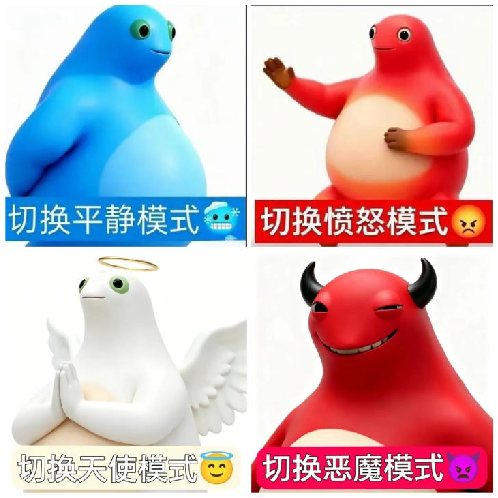
\includegraphics[width=203.32bp,height=0.76\textheight,keepaspectratio]{figures/chapter07/figure07_1.pdf}
  \renewcommand{\thefigure}{7.1}
  \caption{一些不同模式的异色奶蛙形象}
  \label{fig:07-1}
\end{figure}


\subsubsection{（2）植奶、僵奶}

B 站 up 主暖气杀手 AAA 所制作的《植奶大战僵龙》系列，无疑是奶蛙爆火的强力引擎之一。其通过将奶蛙和 PVZ 结合，成功做出多款百万播放视频。~(见\figref{fig:07-2})

% !TEX root = ../../main.tex
\begin{figure}[H]
  \centering
  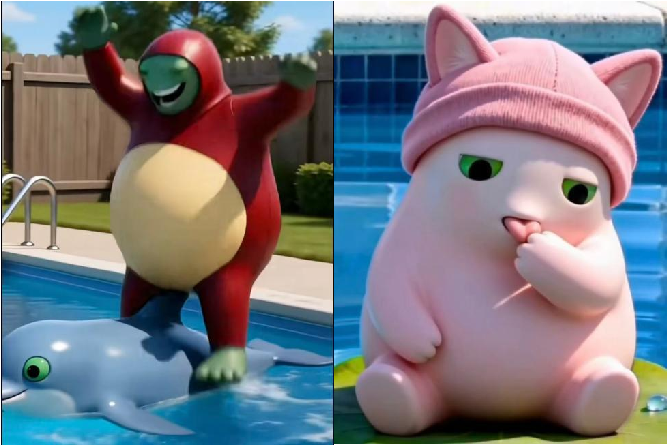
\includegraphics[width=272.48bp,height=0.76\textheight,keepaspectratio]{figures/chapter07/figure07_2.pdf}
  \renewcommand{\thefigure}{7.2}
  \caption{《植奶大战僵龙》系列视频中的海豚僵奶和猫尾奶形象}
  \label{fig:07-2}
\end{figure}


\subsubsection{（3）其他}

其他大部分换皮奶蛙都是用图标、封面等进行换皮，举例如下。~(见\figref{fig:07-3})

\clearpage
% Source PDF page 16.
% !TEX root = ../../main.tex
\begin{figure}[H]
  \centering
  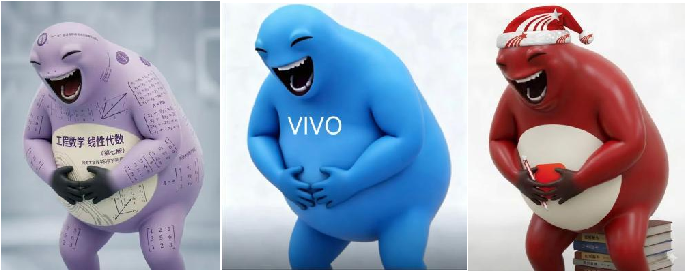
\includegraphics[width=280.02bp,height=0.76\textheight,keepaspectratio]{figures/chapter07/figure07_3.pdf}
  \renewcommand{\thefigure}{7.3}
  \caption{线代课本奶蛙（左） VIVO 奶蛙（中） 学习通奶蛙（右）}
  \label{fig:07-3}
\end{figure}


\subsection{二、异形奶蛙}

异形奶蛙指的是丢失大量形体特征，但是仍然保留眼睛和大笑的变种奶蛙。

\subsubsection{（1）奶蛋}

% !TEX root = ../../main.tex
\begin{figure}[H]
  \centering
  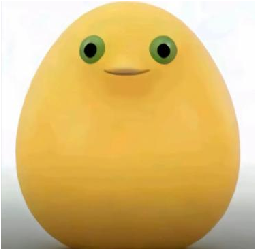
\includegraphics[width=104.28bp,height=0.76\textheight,keepaspectratio]{figures/chapter07/figure07_4.pdf}
  \renewcommand{\thefigure}{7.4}
  \caption{奶蛋的形象}
  \label{fig:07-4}
\end{figure}


\textbf{奶蛋（Milk Egg）}，将奶蛙简化到极致的产物。~(见\figref{fig:07-4})

在 B 站 up 主奶史\_所制作的《选择你的奶伴》系列视频中高频出现，与衍生语“安迪”高频结伴出现，几乎从无败绩。因此产生了“奶蛋轮椅”的说法，把“安迪”等价空耳为“俺无敌”。

现在奶蛋已经默认为奶伴中的至强者之一，\textbf{拥有强大的运气和极为逆天的能力}（包括但不限于空间转移/转变、时间加速、召唤陨石、催眠洗脑）。“安迪”一出，谁与争锋。但在一些日常向作品中，奶蛋不会表现出其实力。

\subsubsection[（2）奶狗\&奶屎、奶鸡、奶鼠\&奶粉、奶茶、豆奶等]{（2）奶狗\&奶屎、奶鸡、奶鼠\&奶粉、奶茶、豆奶等~(见\figref{fig:07-5})}

% !TEX root = ../../main.tex
\begin{figure}[H]
  \centering
  
\includegraphics[width=199.14bp,height=0.76\textheight,keepaspectratio]{figures/chapter07/figure07_5.pdf}
  \renewcommand{\thefigure}{7.5}
  \caption{奶狗（左）和奶屎（右）的形象}
  \label{fig:07-5}
\end{figure}


\textbf{奶狗（Milk Dog）}由于其蠢萌的形象，从十二奶肖中脱颖而出。智商较低，有敏锐的嗅觉，拥有特有动作打滚转圈大笑。

值得注意的是，单只奶狗的能力虽然非常弱，但是一群奶狗的能力将得到显著提升。在奶狗极度愤怒并且拥有项链的情况下，其能够使用召唤术召唤数只小奶狗为自己作战，两只小奶狗合作的威力就能够接近于奶蛙。

\clearpage
% Source PDF page 17.
在某些情况下，奶狗能够使用嗅觉寻找奶蛋，来短暂获得奶蛋的无敌能力。~(见\figref{fig:07-6})

% !TEX root = ../../main.tex
\begin{figure}[H]
  \centering
  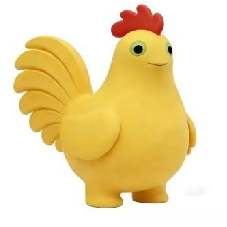
\includegraphics[width=237.8bp,height=0.76\textheight,keepaspectratio]{figures/chapter07/figure07_6.pdf}
  \renewcommand{\thefigure}{7.6}
  \caption{召唤出四只小奶狗的奶狗}
  \label{fig:07-6}
\end{figure}


\textbf{奶屎（Milk Shit）}是与奶狗绑定的形象。可以由奶狗的体内排出，具有吸引奶狗的能力（毕竟狗改不了吃奥利给嘛）。一般没有移动能力，会对身边的奶伴大笑。但在一些作品中，可以长出小短腿进行缓慢的移动。

% !TEX root = ../../main.tex
\begin{figure}[H]
  \centering
  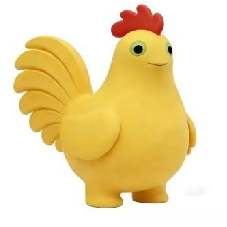
\includegraphics[width=177.31bp,height=0.76\textheight,keepaspectratio]{figures/chapter07/figure07_7.pdf}
  \renewcommand{\thefigure}{7.7}
  \caption{奶鼠（左）和奶粉（右）的形象}
  \label{fig:07-7}
\end{figure}


\textbf{奶鸡（Milk Hen）}从十二奶肖中脱颖而出的原因并不是造型，而是和奶蛋有着现实逻辑的强相关性。奶鸡具有一定的滑翔和缓降能力，可以进行奶蛋的生产。~(见\figref{fig:07-7})

% !TEX root = ../../main.tex
\begin{figure}[H]
  \centering
  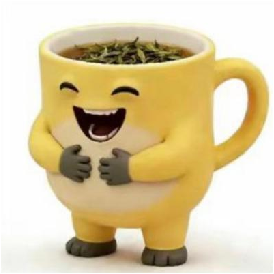
\includegraphics[width=111.93bp,height=0.76\textheight,keepaspectratio]{figures/chapter07/figure07_8.pdf}
  \renewcommand{\thefigure}{7.8}
  \caption{奶茶的形象}
  \label{fig:07-8}
\end{figure}


\textbf{奶鼠（Milk Rat）}由于其可爱萌趣的形象，从十二奶肖中脱颖而出。情商较低，常常因为做嘲讽动作而被远程攻击手段弄翻车，拥有特有语音“奶鼠奶鼠”。~(见\figref{fig:07-8})

\textbf{奶粉（Pink Naiwa）}是与奶鼠绑定的形象。除了身体颜色外，没有与正常奶蛙的明显区别，一般认为其是奶蛙族的雌性个体。其拥有\textbf{必定能全方位克制奶鼠并一定使其吃瘪的能力}（人称“奶鼠最严厉的母亲”）。

\clearpage
% Source PDF page 18.

% !TEX root = ../../main.tex
\begin{figure}[H]
  \centering
  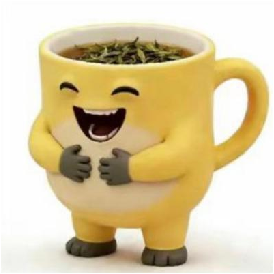
\includegraphics[width=111.93bp,height=0.76\textheight,keepaspectratio]{figures/chapter07/figure07_9.pdf}
  \renewcommand{\thefigure}{7.9}
  \caption{奶茶的形象}
  \label{fig:07-9}
\end{figure}


\textbf{奶茶（Milk Teacup）}常常作为饮品以复数形式出现。和奶蛋的关系貌似很好。~(见\figref{fig:07-9})

% !TEX root = ../../main.tex
\begin{figure}[H]
  \centering
  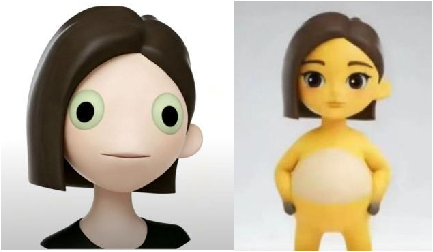
\includegraphics[width=176.8bp,height=0.76\textheight,keepaspectratio]{figures/chapter07/figure07_10.pdf}
  \renewcommand{\thefigure}{7.10}
  \caption{豆奶的原型（左）和经典形象（右）}
  \label{fig:07-10}
\end{figure}


\textbf{豆奶（Nai Doubao）}，豆包和奶蛙的结合体。由于豆包被大家默认为能上桌的 AI 中的最弱档次，于是就和奶龙糖糖联合，形成了豆奶的前身。在奶蛙热度飙升之后，豆包和奶蛙结合形成了豆奶。拥有豆包特有的大笑声音。~(见\figref{fig:07-10})

以上经典形象及其性格特点多在 B 站 up 主奶史\_所制作的《选择你的奶伴》系列中成功深入人心，为奶蛙世界观奠定了根本性的基础。

\subsubsection{（3）奶蛙娘}

% !TEX root = ../../main.tex
\begin{figure}[H]
  \centering
  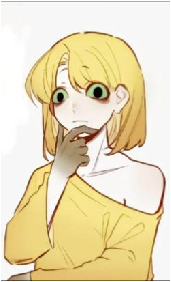
\includegraphics[width=188.63bp,height=0.76\textheight,keepaspectratio]{figures/chapter07/figure07_11.pdf}
  \renewcommand{\thefigure}{7.11}
  \caption{“最绝的角色设计”}
  \label{fig:07-11}
\end{figure}


奶蛙最经典的娘化形象之一（搜不到原画师 qwq）。~(见\figref{fig:07-11})

由于奶蛙的手是黑色的，奶蛙娘的手也是黑色的。由此产生了一个有趣的关联梗：在游戏《魔法少女的魔女审判》中，魔女化的魔法少女的手也会变黑。因此，可以把奶蛙看作奶蛙娘魔奶化后的残骸。~(见\figref{fig:07-12})

\clearpage
% Source PDF page 19.
% !TEX root = ../../main.tex
\begin{figure}[H]
  \centering
  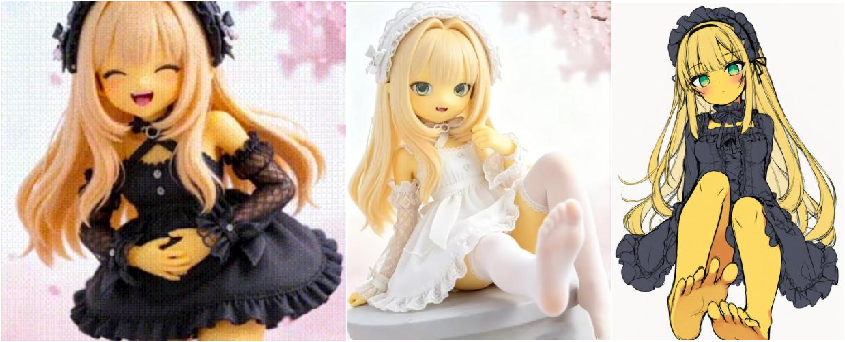
\includegraphics[width=188.63bp,height=0.76\textheight,keepaspectratio]{figures/chapter07/figure07_12.pdf}
  \renewcommand{\thefigure}{7.12}
  \caption{“最绝的角色设计”}
  \label{fig:07-12}
\end{figure}


\subsubsection{（4）奶蝠}

% !TEX root = ../../main.tex
\begin{figure}[H]
  \centering
  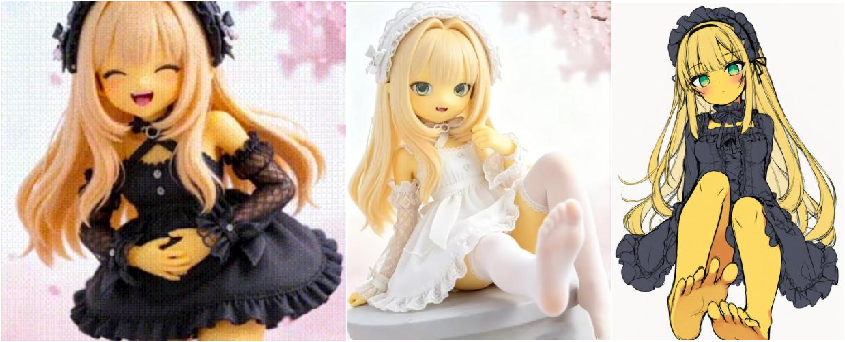
\includegraphics[width=129.88bp,height=0.76\textheight,keepaspectratio]{figures/chapter07/figure07_13.pdf}
  \renewcommand{\thefigure}{7.13}
  \caption{奶正太的形象}
  \label{fig:07-13}
\end{figure}


奶蛙最经典的娘化形象之一，二创最多最神的娘化奶蛙形象。辣眼本《奶莉的诞生》和辣眼 galgame《见习的幸福天使：奶福》采用的就是奶蝠的形象。~(见\figref{fig:07-13})

奶蝠一般以黑色洛丽塔少女的模样出现，本体是一只吸血鬼奶蛙。奶蝠的本体（即吸血鬼奶蛙）具有黑色的巨型翅膀、尖锐的牙齿和又长又尖的耳朵，具有一定的飞行能力。我们姑且认为奶蝠不会随着外貌的变化改变性别。

\subsubsection{（5）奶正太}

% !TEX root = ../../main.tex
\begin{figure}[H]
  \centering
  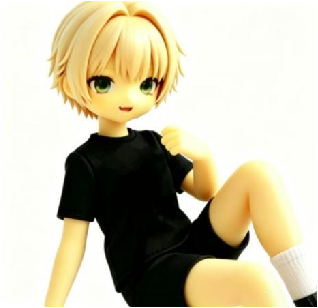
\includegraphics[width=308.28bp,height=0.76\textheight,keepaspectratio]{figures/chapter07/figure07_14.pdf}
  \renewcommand{\thefigure}{7.14}
  \caption{奶龙娘的形象}
  \label{fig:07-14}
\end{figure}


奶蛙的正太形象，和奶蝠的定位类似。~(见\figref{fig:07-14})

\clearpage
% Source PDF page 20.
\subsubsection{（6）奶龙娘}

% !TEX root = ../../main.tex
\begin{figure}[H]
  \centering
  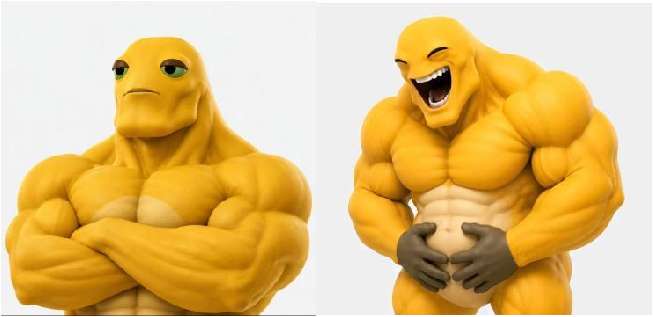
\includegraphics[width=308.28bp,height=0.76\textheight,keepaspectratio]{figures/chapter07/figure07_15.pdf}
  \renewcommand{\thefigure}{7.15}
  \caption{奶龙娘的形象}
  \label{fig:07-15}
\end{figure}


更偏向奶龙的经典娘化形象之一。~(见\figref{fig:07-15})

\subsubsection{（7）奶蛙妹}

% !TEX root = ../../main.tex
\begin{figure}[H]
  \centering
  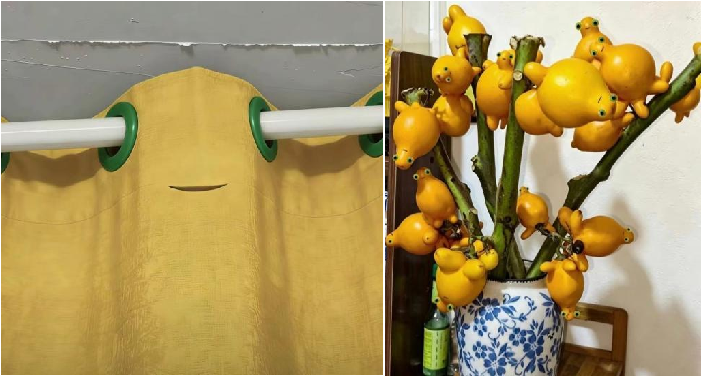
\includegraphics[width=286.45bp,height=0.76\textheight,keepaspectratio]{figures/chapter07/figure07_16.pdf}
  \renewcommand{\thefigure}{7.16}
  \caption{生活中的奶帘（左）和奶五味子盆景（右）}
  \label{fig:07-16}
\end{figure}


画风备受好评的新生代奶蛙娘化形象。作者为 ality5s（小红书）。~(见\figref{fig:07-16})

\subsubsection{（8）西格玛奶蛙}

% !TEX root = ../../main.tex
\begin{figure}[H]
  \centering
  
\includegraphics[width=128.86bp,height=0.76\textheight,keepaspectratio]{figures/chapter07/figure07_17.pdf}
  \renewcommand{\thefigure}{7.17}
  \caption{正在捧腹大笑的 deepseek 鲸鱼}
  \label{fig:07-17}
\end{figure}


奶蛙的硬汉形象，西格玛效果套用在奶蛙身上的产物。~(见\figref{fig:07-17})

\clearpage
% Source PDF page 21.
\subsubsection{（9）现实幻视}

生活中和奶蛙形象神似的物品，较为稀有。~(见\figref{fig:07-18})

% !TEX root = ../../main.tex
\begin{figure}[H]
  \centering
  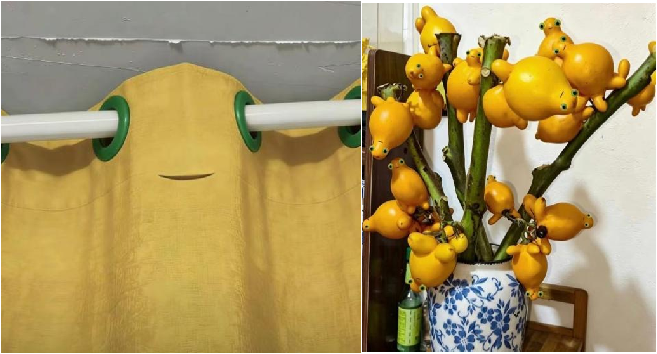
\includegraphics[width=268.09bp,height=0.76\textheight,keepaspectratio]{figures/chapter07/figure07_18.pdf}
  \renewcommand{\thefigure}{7.18}
  \caption{生活中的奶帘（左）和奶五味子盆景（右）}
  \label{fig:07-18}
\end{figure}


\subsubsection{（10）其他 AI 的奶化形象}

作为奶蛙的助推者，除了豆包形成的豆奶外，其他 AI 也受到了奶化。我们在这里以 deepseek、OpenAI、Anthropic、Grok 等为典型代表进行展示。~(见\figref{fig:07-19}, \figref{fig:07-20}, \figref{fig:07-21}, \figref{fig:07-22})

% !TEX root = ../../main.tex
\begin{figure}[H]
  \centering
  
\includegraphics[width=232.59bp,height=0.76\textheight,keepaspectratio]{figures/chapter07/figure07_19.pdf}
  \renewcommand{\thefigure}{7.19}
  \caption{“奶蛋神力由来的传说”}
  \label{fig:07-19}
\end{figure}


% !TEX root = ../../main.tex
\begin{figure}[H]
  \centering
  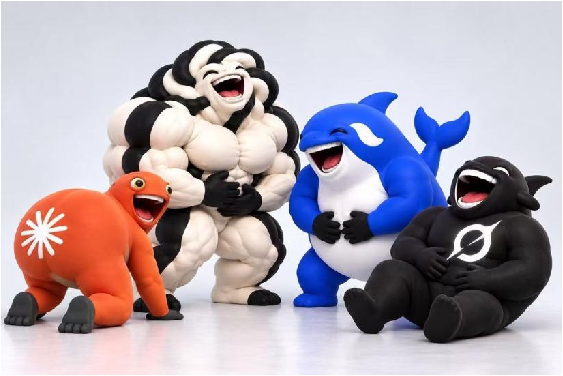
\includegraphics[width=229.53bp,height=0.76\textheight,keepaspectratio]{figures/chapter07/figure07_20.pdf}
  \renewcommand{\thefigure}{7.20}
  \caption{奶工智能四巨头}
  \label{fig:07-20}
\end{figure}


% !TEX root = ../../main.tex
\begin{figure}[H]
  \centering
  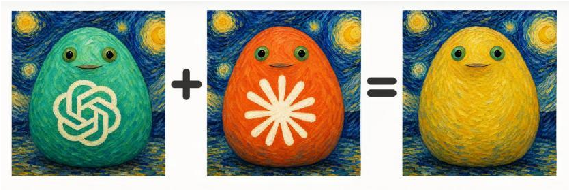
\includegraphics[width=251.97bp,height=0.76\textheight,keepaspectratio]{figures/chapter07/figure07_21.pdf}
  \renewcommand{\thefigure}{7.21}
  \caption{奶菜的形象（左）和奶葡的形象（右）}
  \label{fig:07-21}
\end{figure}


\clearpage
% Source PDF page 22.
% !TEX root = ../../main.tex
\begin{figure}[H]
  \centering
  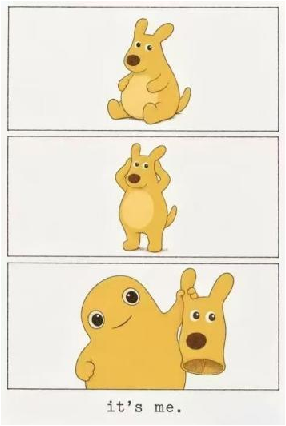
\includegraphics[width=116.72bp,height=0.76\textheight,keepaspectratio]{figures/chapter07/figure07_22.pdf}
  \renewcommand{\thefigure}{7.22}
  \caption{伪装成美团袋鼠的奶蛙}
  \label{fig:07-22}
\end{figure}


\subsubsection{（11）其他}

主要为生活中物品奶龙化的样子。由于篇幅原因，仅在这里举两例。~(见\figref{fig:07-23})

% !TEX root = ../../main.tex
\begin{figure}[H]
  \centering
  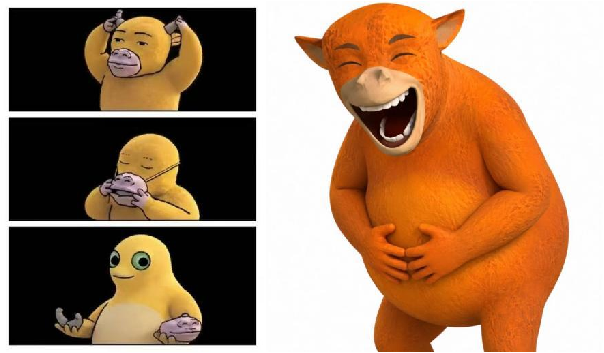
\includegraphics[width=251.97bp,height=0.76\textheight,keepaspectratio]{figures/chapter07/figure07_23.pdf}
  \renewcommand{\thefigure}{7.23}
  \caption{奶菜的形象（左）和奶葡的形象（右）}
  \label{fig:07-23}
\end{figure}


\subsection{三、主要客串角色}

\subsubsection{（1）美团袋鼠}

因为肥嘟嘟的颜色与奶蛙相近，常常与奶蛙联动出场。~(见\figref{fig:07-24})

% !TEX root = ../../main.tex
\begin{figure}[H]
  \centering
  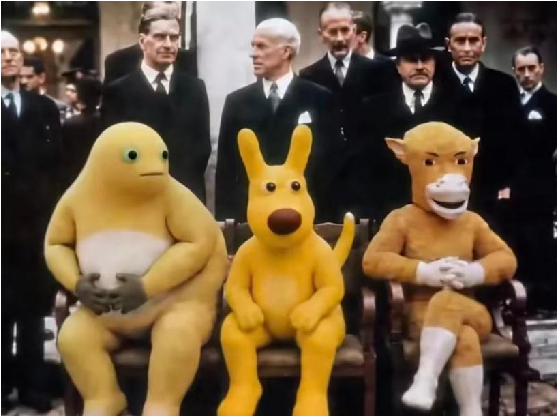
\includegraphics[width=116.72bp,height=0.76\textheight,keepaspectratio]{figures/chapter07/figure07_24.pdf}
  \renewcommand{\thefigure}{7.24}
  \caption{伪装成美团袋鼠的奶蛙}
  \label{fig:07-24}
\end{figure}


\clearpage
% Source PDF page 23.
\subsubsection{（2）牛来、牛来妈}

因为牛来妈的颜色与奶蛙相近，而且牛来和奶蛙抽象程度平分秋色，因此两母子和奶蛙也常常联动出场。~(见\figref{fig:07-25}, \figref{fig:07-26})

% !TEX root = ../../main.tex
\begin{figure}[H]
  \centering
  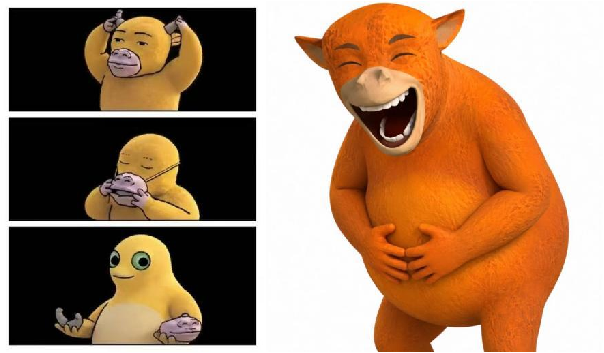
\includegraphics[width=246.36bp,height=0.76\textheight,keepaspectratio]{figures/chapter07/figure07_25.pdf}
  \renewcommand{\thefigure}{7.25}
  \caption{伪装成牛来妈的奶蛙（左）和捧腹大笑的牛来（右）}
  \label{fig:07-25}
\end{figure}


% !TEX root = ../../main.tex
\begin{figure}[H]
  \centering
  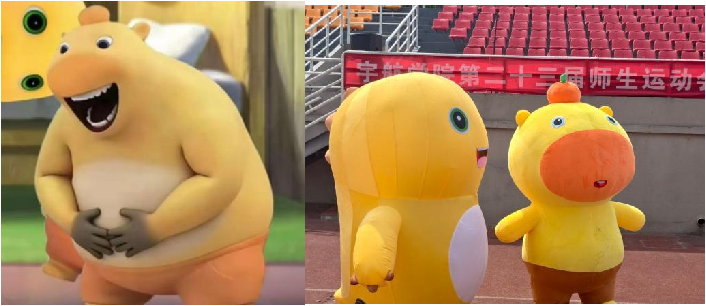
\includegraphics[width=227.8bp,height=0.76\textheight,keepaspectratio]{figures/chapter07/figure07_26.pdf}
  \renewcommand{\thefigure}{7.26}
  \caption{恶搞历史照片：雅尔糖会议三巨头}
  \label{fig:07-26}
\end{figure}


\subsubsection{（3）熊大、熊二}

因为熊二颜色与奶蛙相近，而且熊大有“轻松绷住”、“绷不住了”的梗和奶蛙大笑高度契合，因此两兄弟和奶蛙有时也会联动出场，次数较少。~(见\figref{fig:07-27})

% !TEX root = ../../main.tex
\begin{figure}[H]
  \centering
  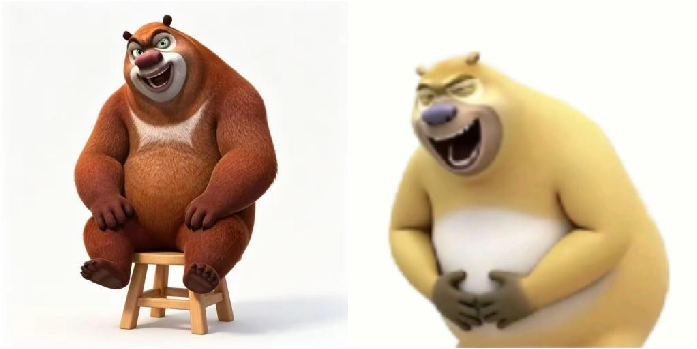
\includegraphics[width=102.85bp,height=0.76\textheight,keepaspectratio]{figures/chapter07/figure07_27.pdf}
  \renewcommand{\thefigure}{7.27}
  \caption{捧腹大笑的蕾雅}
  \label{fig:07-27}
\end{figure}


\clearpage
% Source PDF page 24.
\subsubsection{（4）水豚噜噜}

因为噜噜颜色与奶蛙相近，因此和奶蛙有时也会联动出场，次数较少。~(见\figref{fig:07-28})

% !TEX root = ../../main.tex
\begin{figure}[H]
  \centering
  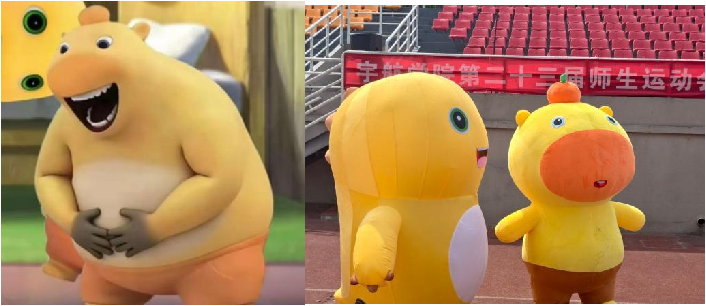
\includegraphics[width=90.41bp,height=0.76\textheight,keepaspectratio]{figures/chapter07/figure07_28.pdf}
  \renewcommand{\thefigure}{7.28}
  \caption{今天，仁者安迪就要捧他的最后一腹！}
  \label{fig:07-28}
\end{figure}


\subsubsection{（5）说的道理}

由于电棍发出的的神秘动静，说的道理拥有多种唐笑，而且作为动物园的一代抽象宗师，道理经常夺舍其他人，绝对有资格驾驭奶蛙的力量。

道理究竟有几种形态呢？~(见\figref{fig:07-29})

% !TEX root = ../../main.tex
\begin{figure}[H]
  \centering
  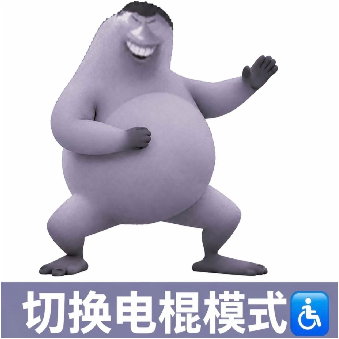
\includegraphics[width=138.45bp,height=0.76\textheight,keepaspectratio]{figures/chapter07/figure07_29.pdf}
  \renewcommand{\thefigure}{7.29}
  \caption{道理奶蛙}
  \label{fig:07-29}
\end{figure}


\subsubsection{（6）绿猪}

愤怒的小鸟中的主要敌人。由于其在玩家失败时的嘲讽笑容过于魔性，形成了一套使用频率较高的绿猪笑笑表情包。而既然绿猪以笑出圈，就自然而然地和奶蛙强强联合，形成了奶蛙的绿猪模式。~(见\figref{fig:07-30})

% !TEX root = ../../main.tex
\begin{figure}[H]
  \centering
  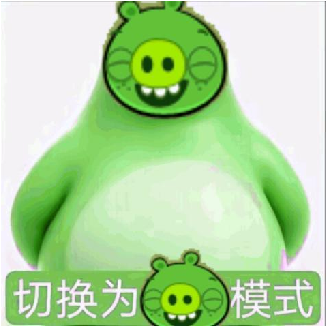
\includegraphics[width=133.25bp,height=0.76\textheight,keepaspectratio]{figures/chapter07/figure07_30.pdf}
  \renewcommand{\thefigure}{7.30}
  \caption{绿猪奶蛙}
  \label{fig:07-30}
\end{figure}


\clearpage
% Source PDF page 25.

\subsection{四、次要客串角色}

次要客串角色的定义是：在一定的圈子内拥有奶之名号，但是并没有像主要客串角色那样破圈被大量使用于表情包传播、二创制作的角色。

\subsubsection{（1）莲见蕾雅}

莲见蕾雅，视觉小说游戏《魔法少女的魔女审判》中 13 名囚犯少女之一。在游戏二周目中，蕾雅成为了二周目希罗小团体的成员，角色定位类似于一周目艾玛小团体的橘雪莉，结果直接从冷静优雅的明星演员滑坡成了一直糖笑的嘉豪逗比（名场面“嘿嘿，哈哈哈哈\textasciitilde{}”），又是金毛，因此被称为魔裁奶龙。

13 名囚犯少女之一的远野汉娜形象要素更接近奶蛙一点（金发而且眼睛也是绿色的），但她的性格一点不像奶蛙。而明明蕾雅眼睛并不是绿色的，却能凭借堪比奶蛙的糖度脱颖而出，这启示我们：只要糖分够，即使没有奶蛙的外表，也拥有了奶蛙的灵魂。

由于名字里有个“蕾”字，蕾雅还和蕾忍宗有着紧密的联系（握握手握握双手），我们在这里按下不表。~(见\figref{fig:07-31})

% !TEX root = ../../main.tex
\begin{figure}[H]
  \centering
  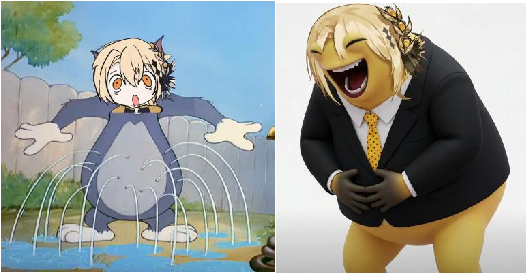
\includegraphics[width=215.05bp,height=0.76\textheight,keepaspectratio]{figures/chapter07/figure07_31.pdf}
  \renewcommand{\thefigure}{7.31}
  \caption{一周目被串串香的蕾雅（左）和二周目捧腹大笑的蕾雅（右）}
  \label{fig:07-31}
\end{figure}


\subsubsection{（2）刹暗天}

刹暗天，港漫《武神》中的中后期主角、港漫《武神终极》中实力最强的终极强者之一（《海虎》三部曲中最强者白首男转世）。以摸鱼摆烂的性格而出名。因为其五级命格“仁者暗帝”可以被空耳为“仁者安迪”，招式暗天车轮拳可以看成奶蛙拳，莫名其妙就和奶蛙扯上了关系。~(见\figref{fig:07-32})

% !TEX root = ../../main.tex
\begin{figure}[H]
  \centering
  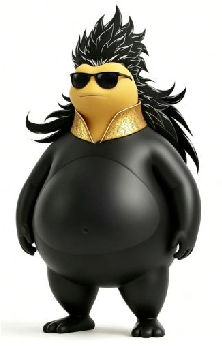
\includegraphics[width=90.41bp,height=0.76\textheight,keepaspectratio]{figures/chapter07/figure07_32.pdf}
  \renewcommand{\thefigure}{7.32}
  \caption{今天，仁者安迪就要捧他的最后一腹！}
  \label{fig:07-32}
\end{figure}


\clearpage
% Source PDF page 26.
% !TEX root = ../../main.tex
\clearpage
\begin{figure}[H]
  \centering
  \phantomsection
  \addcontentsline{lof}{figure}{\protect\numberline{}奶蝠的真身——美丽诱惑下的奶之恶魔}
  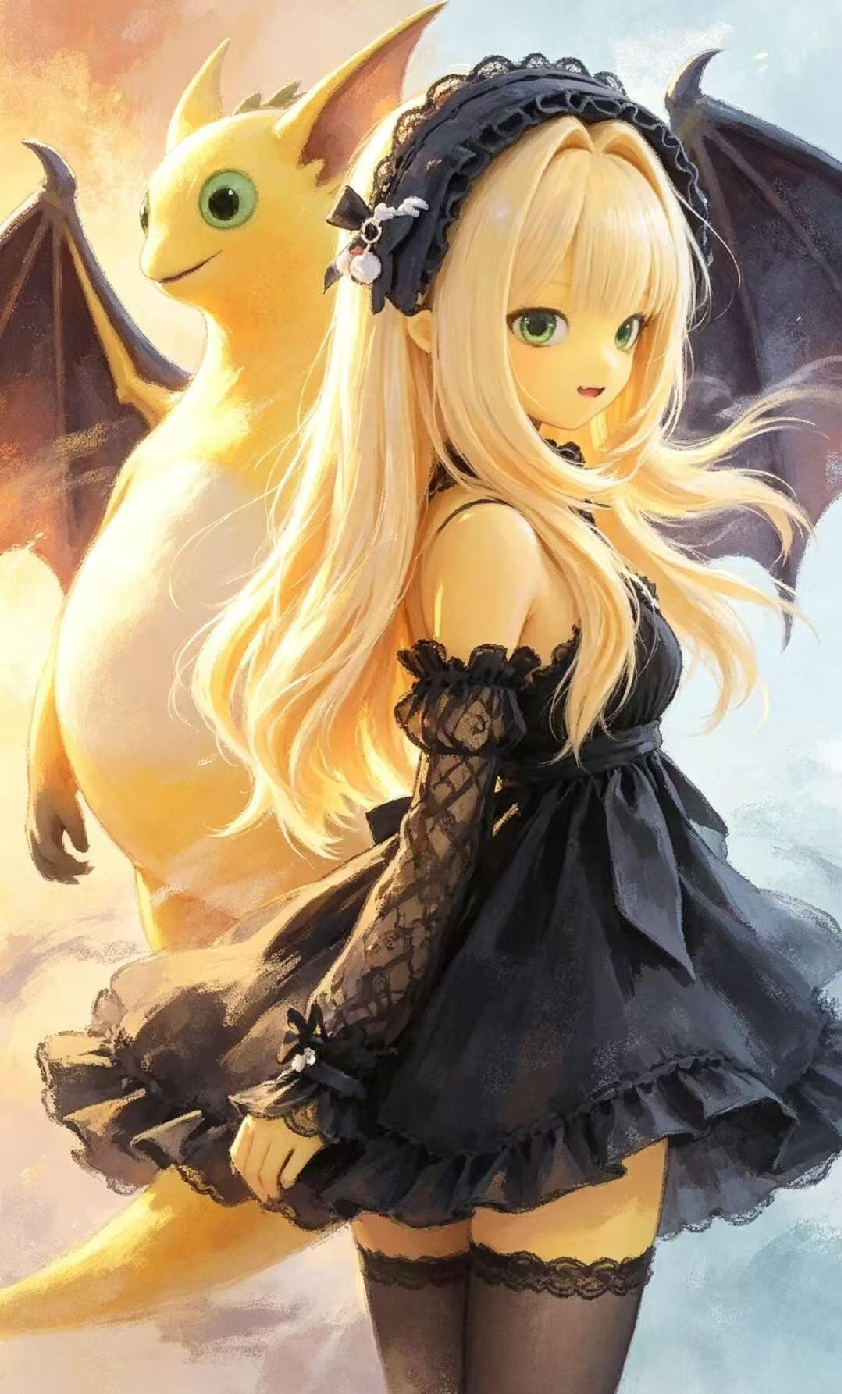
\includegraphics[width=340bp,height=0.90\textheight,keepaspectratio]{figures/chapter07/batPlate.pdf}
  \caption*{奶蝠的真身——美丽诱惑下的奶之恶魔}
\end{figure}
\clearpage


